\documentclass[12pt,a4paper]{article}
\usepackage[utf8]{inputenc}
\usepackage[OT1]{fontenc}
\usepackage{amsmath}
\usepackage{amsfonts}
\usepackage{amssymb}
\usepackage{graphicx}
\usepackage{tikz}
\usepackage{pgfplotstable}
\usepackage{mathtext}

\usepackage[T1]{fontenc}
\usepackage[utf8]{inputenc}
\usepackage[english, bulgarian, russian]{babel}

\usepackage{tikz}
\usepackage{pgfplots}
\usepackage{indentfirst}
\usepackage[export]{adjustbox}
\usepackage{multirow}
\usepackage{geometry} \geometry{verbose,a4paper,tmargin=2cm,bmargin=2cm,lmargin=1.5cm,rmargin=1.5cm}

\graphicspath{{Images/}}
\usepackage[left=2cm,right=2cm,top=2cm,bottom=2cm]{geometry}
\usepackage{wrapfig}
\usepackage{setspace}
\usepackage{indentfirst}
\usepackage{subfigure}

\begin{document}
	
	\begin{titlepage}
		\begin{center}
			\large 	Московский физико-технический институт \\
			\vspace{0.2cm}
			
			\vspace{4.5cm}
			Лабораторная работа № 3.3.4 \\ \vspace{0.2cm}
			\large (Общая физика: электричество и магнетизм) \\ \vspace{0.2cm}
			\LARGE \textbf{Эффект Холла в полупроводниках}
		\end{center}
		\vspace{2.3cm} \large
		
		\begin{center}
			Работу выполнили: \\
			Фитэль Алёна\\
                Попеску Полина\\
                Б06-103
			\vspace{10mm}		
			
		\end{center}
		
		\begin{center} \vspace{60mm}
			г. Долгопрудный \\
			2022 год
		\end{center}
	\end{titlepage}
	
	
	\paragraph*{Цель работы:} измерение подвижности и концентрации носителей заряда в полупроводниках.
	
	\paragraph*{Оборудование:} электромагнит с источником питания, батарейка, амперметр, реостат, цифровой вольтметр, милливеберметр, образцы легированного германия.
	
	\section{Теоретическая справка}
	Суть эффекта Холла состоит в следующем. Пусть через однородную пластину металла вдоль оси $x$ течет ток $I$ (рис. 1).
	
	\begin{wrapfigure}{l}{0.6\textwidth}
		\vspace{-20pt}
		\begin{center}
			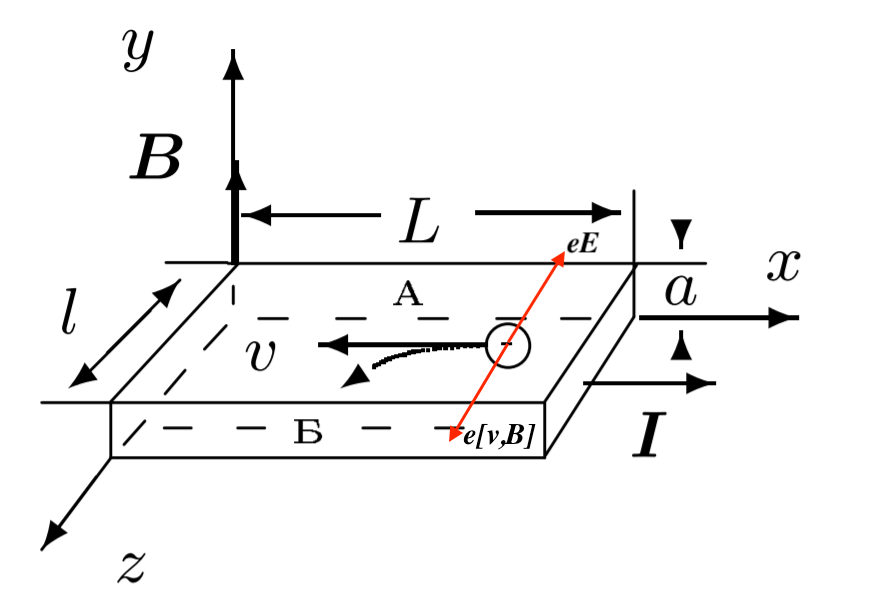
\includegraphics[width=0.7\linewidth]{Holl1.png}
			\label{fig:sdfsafd}
		\end{center}
		\vspace{-20pt}
		\caption{Образец с током в магнитном поле}
	\end{wrapfigure}

	Если эту пластину поместить в магнитное поле, направленное по оси y, то между гранями А и Б появляется разность потенциалов. 
	
	В самом деле, на электрон (для простоты рассматриваем один тип носителей), движущийся со средней скоростью $\langle \vec{v} \rangle$ в электромагнитном поле, действует сила Лоренца:
	
	$$\vec{F}_{л} = -e\vec{E}-e \langle \vec{v} \rangle \times \vec{B},$$
	
	где $e$- абсолютный заряд электрона, $\vec{E}$ - напряженность электрического поля, $\vec{B}$ - индукция магнитного поля.
	
	В проекции на ось $z$ получаем
	
	$$ F_{B}=e | \langle {v_{x}} \rangle | B.$$
	
	Под действием этой силы электроны отклоняются к грани Б, заряжая ее отрицательно. На грани А накапливаются нескомпенсированные положительные заряды. Это приводит к возникновению электрического поля $E_{z}$, направленного от А к Б, которое действует на электроны с силой $F_{E}=eE_{z}$. В установившемся режиме $F_{E}=F_{B}$, поэтому накопление электрических зарядов на боковых гранях пластины прекращается. Отсюда
	
	$$ E_{z}=| \langle {v_{x}} \rangle | B.$$
	
	С этим полем связана разность потенциалов $$U_{AБ}=E_{z}l=| \langle {v_{x}} \rangle | Bl.$$
	
	В этом и состоит эффект Холла.
	
	\
	
	Замечая, что сила тока
	
	$$ I=ne| \langle {v_{x}} \rangle |la,$$
	
	найдем ЭДС Холла:
	
\begin{equation}\label{Rx}
	\mathscr{E}_{X}=U_{AБ}=\dfrac{IB}{nea}=R_{X}\dfrac{IB}{a}
\end{equation}
	
	Константа $R_{X}=\dfrac{1}{ne}$ называется постоянной Холла.
	
	В полупроводниках, когда вклад в проводимость обусловлен и электронами и дырками, выражение для постоянной Холла имеет более сложный вид:
	
	$$R_{X}=\dfrac{nb^{2}_{e}-pb^{2}_{p}}{e(nb_{e}+pb_{p})^{2}},$$
	
	где $n$ и $p$ - концентрации электронов и дырок, $b_{e}$ $b_{p}$ - их подвижности.
	
	\section{Экспериментальная установка.}
	Схема экспериментальной установки показана на рис. 2.
	
	\begin{figure}[h!]
		\centering
		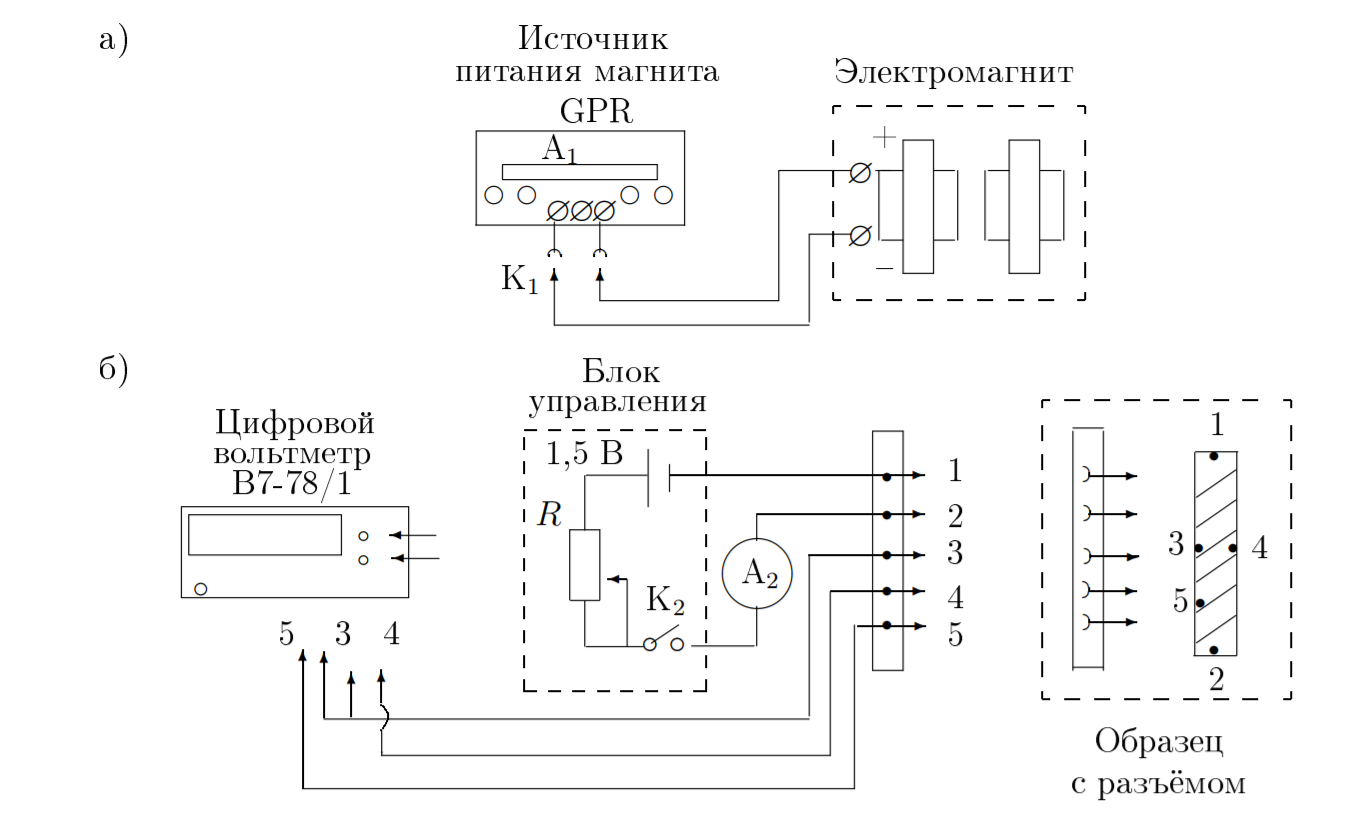
\includegraphics[scale=0.5]{Holl2}
		\caption{Схема установки для исследования эффекта Холла в полупроводниках}
		\label{fig:Holl2}
	\end{figure}
  
  	В зазоре электромагнита (рис. 1а) создаётся постоянное магнитное поле, величину которого можно менять с помощью регуляторов источника питания. Ток измеряется амперметром источника питания $A_{1}$. Разъем $K_{1}$ позволяет менять направление тока в обмотках электромагнита.
  
  	Образец из легированного германия, смонтированный в специальном держателе (рис. 1б), подключается к батарее. При замыкании ключа $K_{2}$ вдоль длинной стороны образца течет ток, величина которого регулируется реостатом $R$ и измеряется миллиамперметром $А_{2}$.
  	
  	В образце с током, помещённом в зазор электромагнита, между контактами 3 и 4 возникает разность потенциалов $U_{34}$, которая измеряется с помощью цифрового вольтметра.
  	
  	Контакты 3 и 4 вследствие неточности подпайки не всегда лежат на одной
  	эквипотенциали, и тогда напряжение между ними связано не только с эффектом
  	Холла, но и с омическим падением напряжения, вызванным протеканием основного тока через образец.
  	
  	Измеряемая разность потенциалов при одном направлении
  	магнитного поля равна сумме ЭДС Холла и омического падения напряжения, а
  	при другом  их разности. В этом случае ЭДС Холла $\mathscr{E}_{X}$ может быть определена как половина алгебраической разности показаний вольтметра, полученных для
  	двух противоположных направлений магнитного поля в зазоре.
  	
  	Можно исключить влияние омического падения напряжения иначе, если при каждом токе через образец измерять напряжение между точками 3 и 4 в отсутствие магнитного поля. При фиксированном токе через образец это дополнительное к ЭДС Холла напряжение $U_{0}$ остается неизменным. От него следует (с учетом
  	знака) отсчитывать величину ЭДС Холла: 
  	
  	$$\mathscr{E}_{X} = U_{34} \pm U_{0}$$. 
  	
  	При таком способе измерения нет необходимости проводить повторные измерения с противоположным направлением магнитного поля.
  	
  	
  	По знаку $\mathscr{E}_{X}$ можно определить характер проводимости - электронный или дырочный. Для этого необходимо знать направление тока в образце и направление
  	магнитного поля.
  	
  	Измерив ток $I$ в образце и напряжение $U_{35}$ между контактами 3 и 5 в отсутствие магнитного поля, можно, зная параметры образца, рассчитать проводимость материала образца по формуле:
  	
  \begin{equation}\label{sigma}
  	\sigma=\dfrac{IL_{35}}{U_{35}al}
  \end{equation}
  	
  	где $L_{35}$ - расстояние между контактами 3 и 5, $a$ - толщина образца, $l$ - его ширина.
  	
  	\section{Ход работы}
  	
  	\begin{enumerate}
  	\item Запишем данные установки:
  	
  	$a=2,2 \; мм,$ $L_{35}=6,0 \;мм,$ $l=7,0 \;мм,$ $SN=75 \;см^{2}\cdot вит$ - площадь сечения контура катушки на число витков в ней.
  	
  	\item Настроим приборы согласно инструкции.
  	
  	\item Запишем предельное значение тока через электромагнит:
  	
  	$$ I_{max}=2,13 \; А.$$
  	
  	\item Исследуем зависимость потока $ \Phi $ магнитного поля в зазоре электромагнита от тока через обмотки магнита. Данные занесём в табл. 1.
  	
  	Индукцию $B$ найдем по формуле
  	
  \begin{equation}\label{}
  	B=\dfrac{\Delta Ф}{SN},
  \end{equation}
  	
  	

   \begin{figure}[h!]
	\centering
	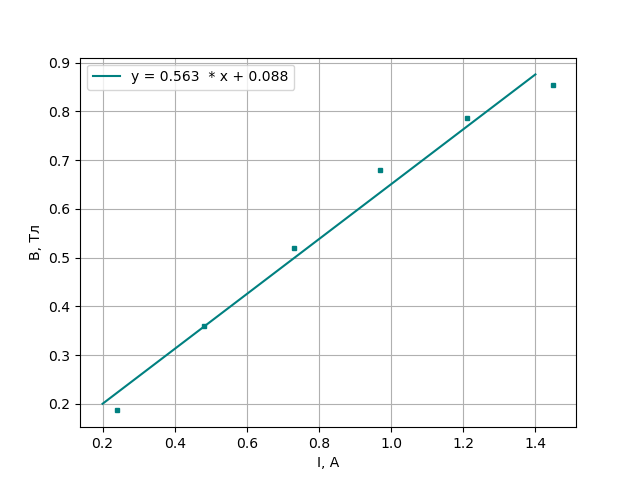
\includegraphics[scale=0.7]{334graph1.png}
	\caption{График зависимости $ B(I_M) $}
\end{figure}

  	
  		
  	
  		\begin{table}[]
  			\caption{Зависимость $B(I_{м})$}
  		\begin{center}
  		\begin{tabular}{|c|c|c|c|} 
  			\hline 
  			№ &  $I_{м}$, A &  $Ф_{0}$, мВб & $Ф$, мВб & $\Delta Ф$, мВб & $B, Тл$  \\ 	\hline
  			
  			1 & 0,24 & 1,4 & 0,019 \\
  			2 & 0,48 & 2,7 & 0,036 \\
  			3 & 0,73 & 3,9 & 0,052 \\
  			4 & 0,97 & 5,1 & 0,068 \\
  			5 & 1,21 & 5,9 & 0,079 \\
  			6 & 1,45 & 6,4 & 0,085\\
  			\hline
  			
  		\end{tabular}
  	\end{center}
  \end{table}

  	По этим данным построим график зависимости $B=B(I_{M})$ (рис. 3).
  	
  	\item Снимем зависимость $U_{34}(I_{м})$ различных токах через образец (табл. 2). А именно, он изменяется от 0,23 до 1,07 мА. При этом в отсутствие магнитного поля вольтметр покажет напряжение $U_{0}$. Результаты занесём в таблицу 2, подписывая сверху $ I, U_0 $  в мА и мкВ соответственно. В последнем опыте изменим направление магнитного поля.

   
   \begin{figure}[h!]
	\centering
	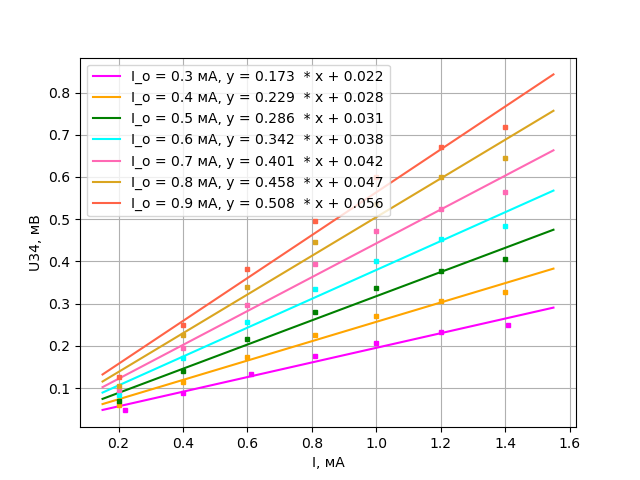
\includegraphics[scale=0.7]{334_graph2.png}
        \caption{График зависимости $U_{34}(I_{м})$}
\end{figure}


\begin{table}[]
\begin{tabular}{|c|cccccccc|c|}
\hline
$ N $ & \multicolumn{1}{c|}{$ I_M, A $} & \multicolumn{1}{c|}{$I, \; U_0 $} & \multicolumn{1}{c|}{$I, \;U_0 $}    & \multicolumn{1}{c|}{$I, \;U_0 $}   & \multicolumn{1}{c|}{$I, \;U_0 $}    & \multicolumn{1}{c|}{$I, \;U_0 $}   & \multicolumn{1}{c|}{$I, \;U_0 $}   & $I, \;U_0 $     & $I, \;U_0 $     \\ \hline
      & \multicolumn{1}{c|}{}           & \multicolumn{1}{c|}{$0,30,  \;3$} & \multicolumn{1}{c|}{$ 0,40,  \;3 $} & \multicolumn{1}{c|}{$  0,50, \;3$} & \multicolumn{1}{c|}{$  0,60,  \;4$} & \multicolumn{1}{c|}{$ 0,70,  \;5$} & \multicolumn{1}{c|}{$ 0,80, \; 5$} & $  0,90,  \;6 $ & $ 0,90,\; -17 $ \\ \hline
      &                                 &                                   &                                     &                                    & $ U34, \; мкВ $                     &                                    &                                    &                 &                 \\ \hline
1     & \multicolumn{1}{c|}{0.20}       & \multicolumn{1}{c|}{50}           & \multicolumn{1}{c|}{63}             & \multicolumn{1}{c|}{73}            & \multicolumn{1}{c|}{88}             & \multicolumn{1}{c|}{100}           & \multicolumn{1}{c|}{110}           & 131             & -139            \\ \hline
2     & \multicolumn{1}{c|}{0.40}       & \multicolumn{1}{c|}{92}           & \multicolumn{1}{c|}{118}            & \multicolumn{1}{c|}{145}           & \multicolumn{1}{c|}{174}            & \multicolumn{1}{c|}{201}           & \multicolumn{1}{c|}{230}           & 256             & -256            \\ \hline
3     & \multicolumn{1}{c|}{0.60}       & \multicolumn{1}{c|}{137}          & \multicolumn{1}{c|}{177}            & \multicolumn{1}{c|}{219}           & \multicolumn{1}{c|}{260}            & \multicolumn{1}{c|}{301}           & \multicolumn{1}{c|}{345}           & 387             & -304            \\ \hline
4     & \multicolumn{1}{c|}{0.80}       & \multicolumn{1}{c|}{171}          & \multicolumn{1}{c|}{228}            & \multicolumn{1}{c|}{285}           & \multicolumn{1}{c|}{338}            & \multicolumn{1}{c|}{399}           & \multicolumn{1}{c|}{451}           & 501             & -512            \\ \hline
5     & \multicolumn{1}{c|}{1.00}       & \multicolumn{1}{c|}{209}          & \multicolumn{1}{c|}{274}            & \multicolumn{1}{c|}{341}           & \multicolumn{1}{c|}{406}            & \multicolumn{1}{c|}{476}           & \multicolumn{1}{c|}{542}           & 605             & -614            \\ \hline
6     & \multicolumn{1}{c|}{1.20}       & \multicolumn{1}{c|}{235}          & \multicolumn{1}{c|}{309}            & \multicolumn{1}{c|}{381}           & \multicolumn{1}{c|}{456}            & \multicolumn{1}{c|}{530}           & \multicolumn{1}{c|}{605}           & 677             & -685            \\ \hline
7     & \multicolumn{1}{c|}{1.40}       & \multicolumn{1}{c|}{0,252}        & \multicolumn{1}{c|}{331}            & \multicolumn{1}{c|}{409}           & \multicolumn{1}{c|}{489}            & \multicolumn{1}{c|}{570}           & \multicolumn{1}{c|}{649}           & 725             & -735            \\ \hline
\end{tabular}
\caption{Результаты измерений $ U_{34} $}
\end{table}


  
 \item Рассчитаем ЭДС Холла и построим на одном графике семейство характеристик $\mathcal{E}_x=f(B)$ при разных токах, определим угловые коэффициенты $k(I)=\Delta \mathcal{E}/ \Delta B$. Построим график $k = f(I)$, рассчитаем угловой коэффициент и по формуле $\mathcal{E}_x= -R_x \cdot \frac{IB}{a}$ рассчитаем постоянную Холла $R_X$\\ 


   \begin{figure}[h!]
	\centering
	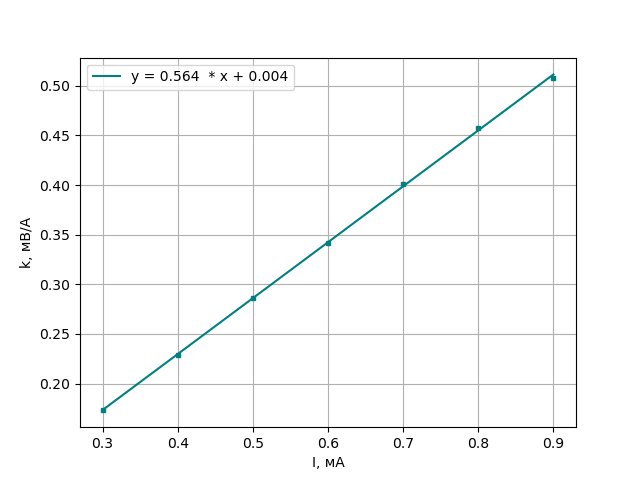
\includegraphics[scale=0.7]{334graph3.png}
        \caption{График зависимости $k(I)$}
\end{figure}



\begin{table}[h!]
\centering
\begin{tabular}{|l|l|l|l|l|l|l|l|}
\hline
$k$, мВ/Вб  & 0.173 & 0.229 & 0.286 & 0.342 & 0.401 & 0.458 & 0.508 \\ \hline
$I$, А & 0.3  & 0.4  & 0.5  & 0.6  & 0.7 & 0.8  & 0.9   \\ \hline
\end{tabular}
\end{table}



\begin{equation*}
    R_x = {\varepsilon_x \over IB}a = {\varepsilon_x\over I \cdot I_M} {I_M \over B}a = {k_2 \over k_1} a = (750 \pm 50) \cdot 10^{-3}{В\cdot м \over Тл\cdot А}
\end{equation*}

 \item

Определим, что наши частицы движутся к клемме №4 образца. Зная направление магнитного поля в электромагните и тока через образец, мы определяем, что наши частицы заряжены отрицательно, т.е. являются электронами.
  
  \item 
  
  Теперь определим концентрацию электронов:
 
\begin{equation}\label{}
   n = {1 \over e R_x} = (8,3 \pm 0,6) \cdot 10^{18} {1\over м^3}
\end{equation}


\item Для определения удельной проводимости выключим источник питания и измерим падение напряжения $U_{35}$ (1 мА)= -4,036 мВ.

\begin{equation}\label{}
\sigma = {IL \over U_{35}al} = 156,6 \pm 3 {1 \over Ом \cdot м}
\end{equation}

\item

По формуле посчитаем подвижность электронов: 

\begin{equation}\label{}
b = {\sigma \over en} = \sigma R_x = (0,12 \pm 0,01) \cdot 10^{-3} {м^2 \over В \cdot с}
\end{equation}

\section{Вывод}

В ходе работы изучено явление Холла на основе образца. 
Также вычислена постоянная Холла для исследуемого образца $R_x = (750 \pm 50) \cdot 10^{-6}{В\cdot м \over Тл\cdot А}\ (\varepsilon \approx 7 \%)$, концентрация носителей заряда $n = (8,3 \pm 0,6) \cdot 10^{21} {1\over м^3}\ (\varepsilon \approx 8\%)$, 
удельная проводимость $\sigma = 156,6 \pm 3 {1 \over Ом \cdot м}\ (\varepsilon \approx 2\%)$ и подвижность носителей заряда $b = 120 \pm 10 {cм^2 \over В \cdot с}\ (\varepsilon \approx 9\%)$. 
Полученные данные могут отличаться от табличных в связи с сильной чувствительностью используемого прибора к нагреву, происходящему при проходе через него тока, и большим количеством примесей в рассматриваемом образце.
 	 
  	
\end{enumerate}
\end{document}